\newpage
\section{Analisi statistica DnsJava}

\subsection{Analisi Statistica Technical Debt}
In \autoref{td_AnalisiDnsJava-tipo} si osserva la dimensione del technical debt rispetto alla tipologia di clone. Questa analisi statistica è confermata dal p-value, ottenuto con il test di Kruskal-Wallis mediante R, che ha un valore inferiore a $2,2 e^{-16}$.
\begin{figure}[htbp]
	\centering
	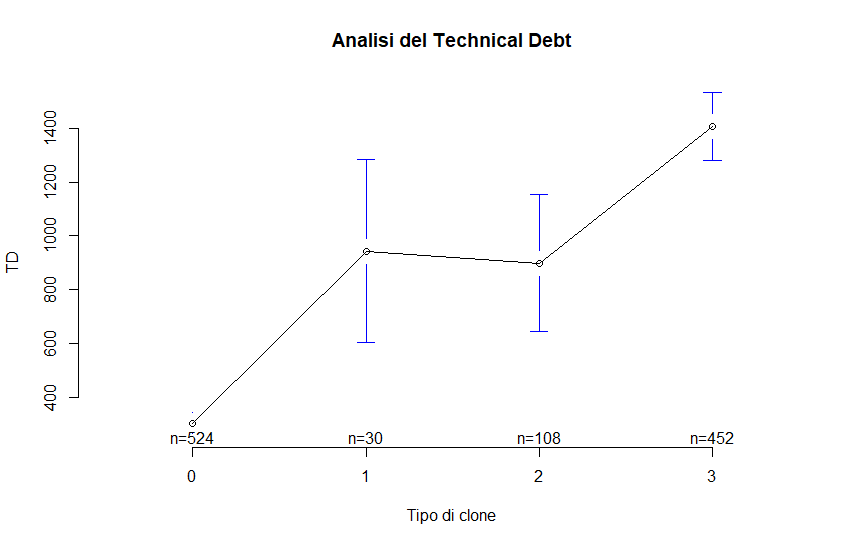
\includegraphics[scale=0.5]{analisi_R/AnalisiDnsJava/1-gplot-td-type.png}
\caption{Analisi statistica Technical Debt}
\label{td_AnalisiDnsJava-tipo}
\end{figure}

In \autoref{td_AnalisiDnsJava-tipo} si rappresenta sull'asse delle ascisse il tipo di clone, indicando con 0 le classi in cui il codice clonato risulta assente. Si riporta, invece, sull'asse delle ordinate il valore del technical debt. Si indica con n il numero delle occorrenze complessive dei cloni di ciascun tipo presenti nelle quattro versioni del progetto. I risultati dell'analisi statistica confermano quanto ipotizzato, ossia che per i cloni di tipo 3 il technical debt risulta maggiore rispetto a quello dei cloni di tipo 1 e 2. L'analisi risulta significativa in quanto le quantità di cloni dei tre tipi risultano confrontabili.
\subsection{Analisi Statistica Code Smells}
In \autoref{codesmell_AnalisiDnsJava-tipo} si mostra la quantità di code smells rispetto alla tipologia di clone. L' analisi statistica è confermata dal p-value, ottenuto con il test di Kruskal-Wallis mediante R, che ha un valore inferiore a $2,2 e^{-16}$. \newpage
\begin{figure}[htbp]
	\centering
	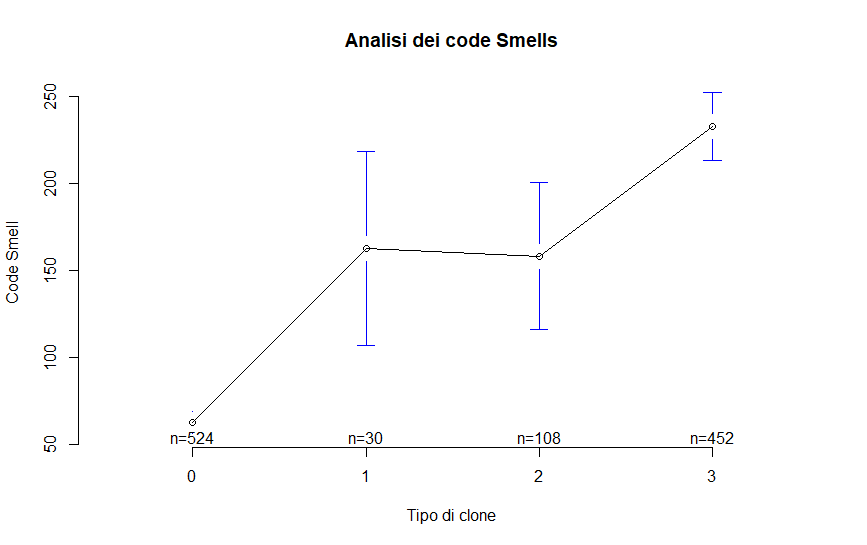
\includegraphics[scale=0.5]{analisi_R/AnalisiDnsJava/2-gplot-codesmell-type.png}
\caption{Analisi statistica Code Smell}
\label{codesmell_AnalisiDnsJava-tipo}
\end{figure}
In \autoref{codesmell_AnalisiDnsJava-tipo}  si rappresenta sull'asse delle ascisse il tipo di clone, indicando con 0 le classi in cui il codice clonato risulta assente. Si riporta, invece, sull'asse delle ordinate il numero di code smells. Si indica con n il numero delle occorrenze dei cloni di ciascun tipo presenti nelle quattro versioni del progetto. L'analisi statistica conferma che per i cloni di tipo 3 la quantità di code smells risulta maggiore rispetto agli altri due tipi di cloni.
\subsection{Analisi Statistica Lunghezza Codice Clonato}
In \autoref{len_AnalisiDnsJava-tipo} si osserva la lunghezza del codice clonato (espressa in LOC) rispetto alla tipologia di clone. L' analisi statistica è confermata dal p-value, ottenuto con il test di Kruskal-Wallis mediante R, che ha un valore inferiore a $2,2 e^{-16}$. \newpage
\begin{figure}[htbp]
	\centering
	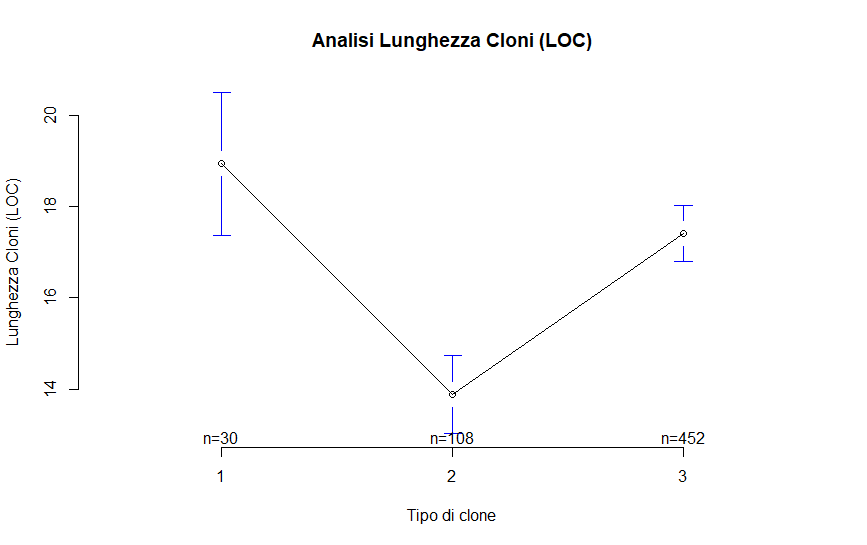
\includegraphics[scale=0.5]{analisi_R/AnalisiDnsJava/3-gplot-len-type.png}
\caption{Analisi statistica Lunghezza Codice Clonato }
\label{len_AnalisiDnsJava-tipo}
\end{figure}
In \autoref{len_AnalisiDnsJava-tipo} si riporta sull'asse delle ascisse il tipo di clone e sull'asse delle ordinate il numero di LOC. Si nota, anche in questo caso, che i cloni di tipo 3 hanno in media numero di LOC maggiore rispetto ai cloni di tipo 1 e 2.